\begin{appendices}
%\addtocontents{toc}{\protect\setcounter{tocdepth}{0}}
\chapter{Procrustes Problem}
The orthogonal Procrustes problem is defined as finding the orthogonal matrix $\Omega$ which transform the matrix $A$ to $B$ or closest to $B$. Mathematically, it is defined:
\begin{eqnarray}
\Omega A&=&B \\
\Omega A-B&=&0 \\ \nonumber
\|\Omega A-B\|&=&0 \\ \nonumber
\mbox{or} \quad \mbox{min} \|\Omega A-B\|&&  \\ \nonumber
\mbox{subject to} \quad \Omega^{T}\Omega=I \\ \nonumber
\mbox{where} \quad \|.\| \quad \mbox{is Frobenius norm}
\end{eqnarray}
Frobernius norm can be calculated using trace:
\begin{eqnarray}
\|\Omega A-B\|^{2}=\mbox{trace}(A^{T}A-2\Omega^{T}A^{T}B+B^{T}B)
\end{eqnarray}
It is obvious that minimizing the frobernius norm is equivalent to maximizing the trace$(\Omega^{T}A^{T}B)$. By decomposing $A^{T}B$ into its SVD component, then matrix $\Omega$ can be determined,
\begin{eqnarray}
\mbox{trace}(\Omega^{T} A^{T} B)&=&\mbox{trace}(\Omega^{T} U \Sigma V^{T}) \\ \nonumber
&=&\mbox{trace}(V^{T}\Omega^{T} U \Sigma) \\ \nonumber
&\leq& \sum_{i} \sigma_{i}.
\end{eqnarray}
The trace is maximum if $\Omega=U V^{T}$ where $[U \Sigma V]=\mbox{SVD}(A^{T}B)$. 
\chapter{Active Set Run}
The data of run using the active set algorithm is displayed in this appendix. The third column is the objective function and the fourth column is the maximum constraint violation. By the end of iteration, the objective function goes to zero and the violation constraint goes to zero as well. The inputs of the algorithm are the definition of the objective function and the inequality constraint as described in the previous section.
\begin{figure}[h!]
\centering
 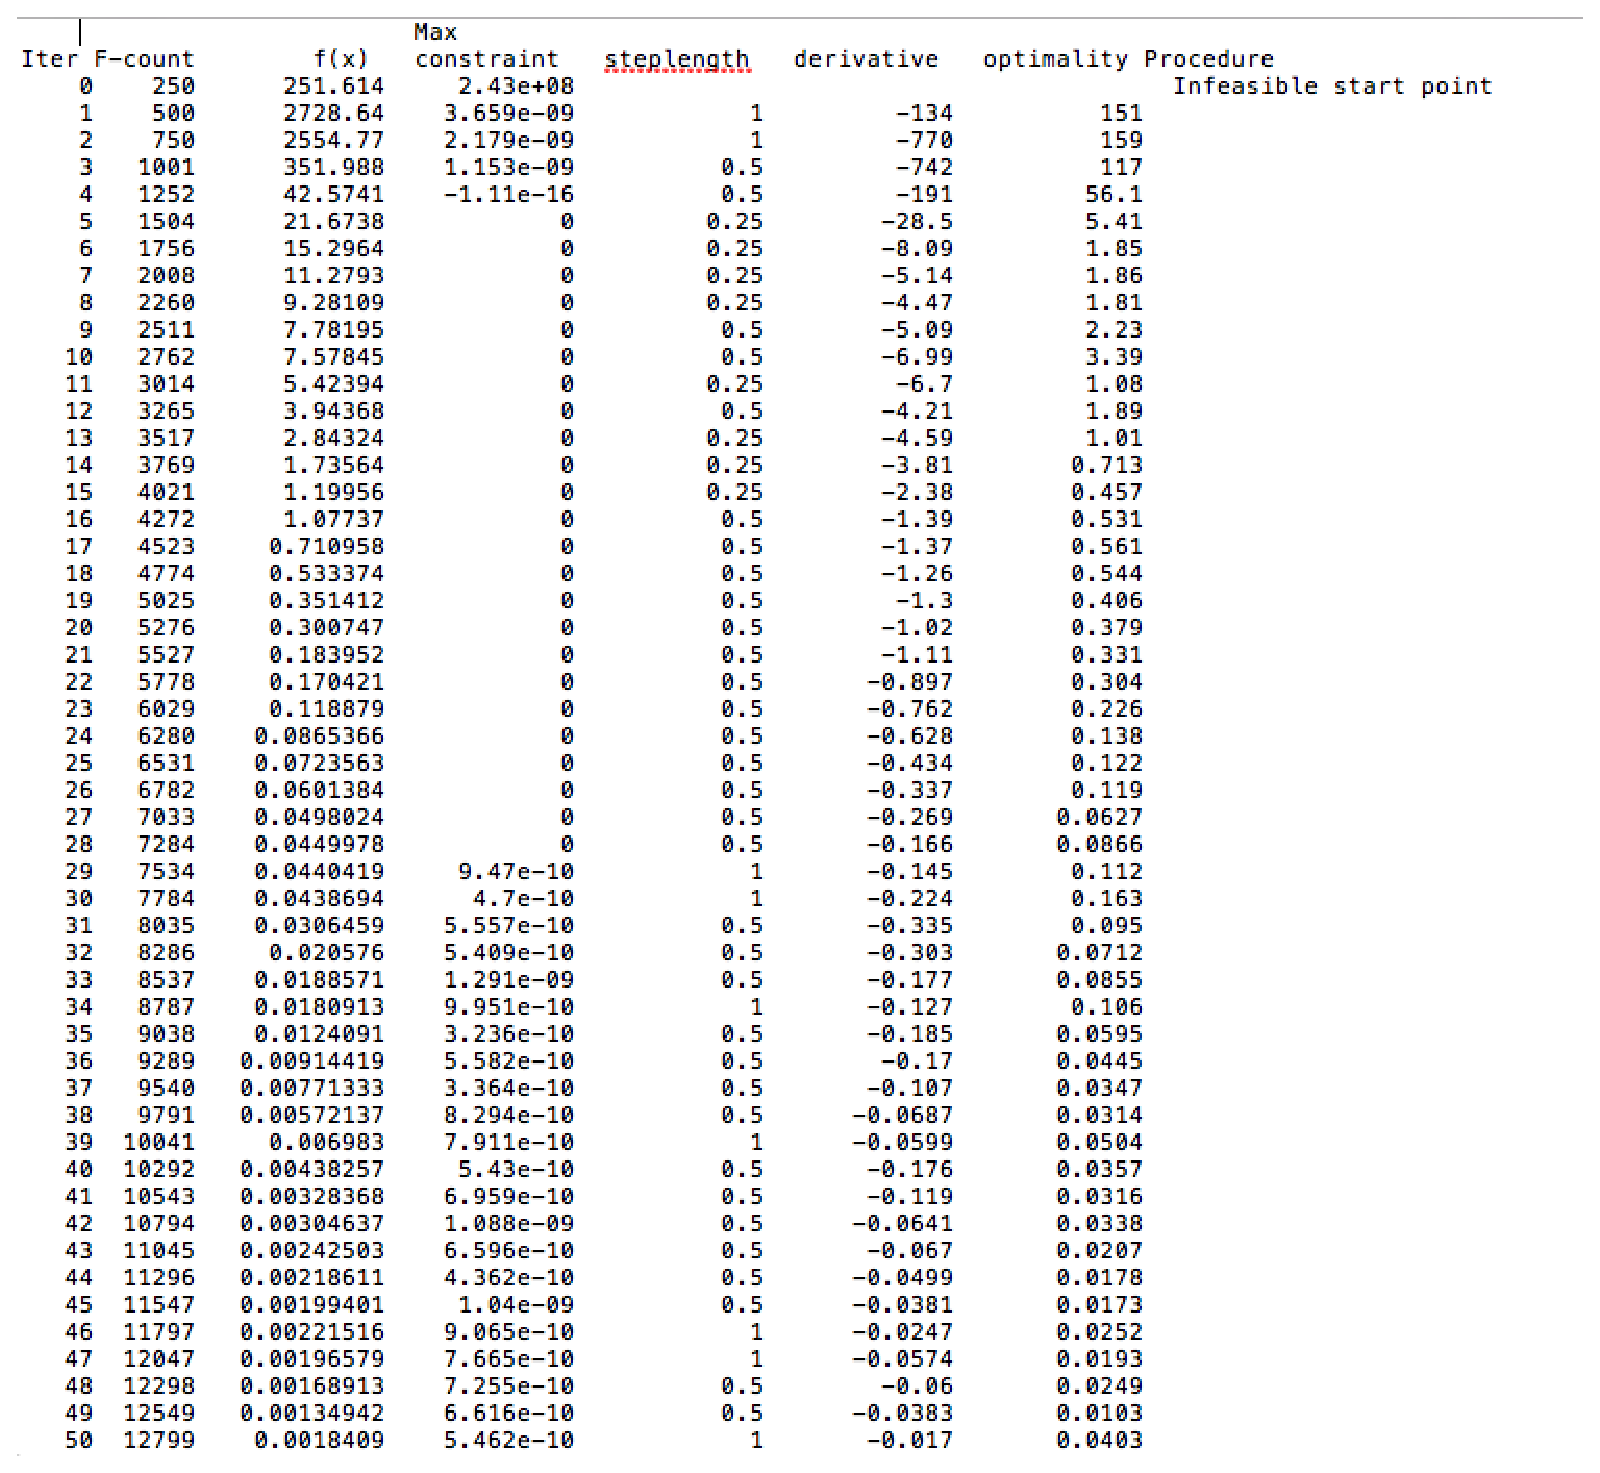
\includegraphics[width=.8\textwidth]{rundata}
\label{fig:rundata}
\end{figure}
\begin{figure}[h!]
\centering
 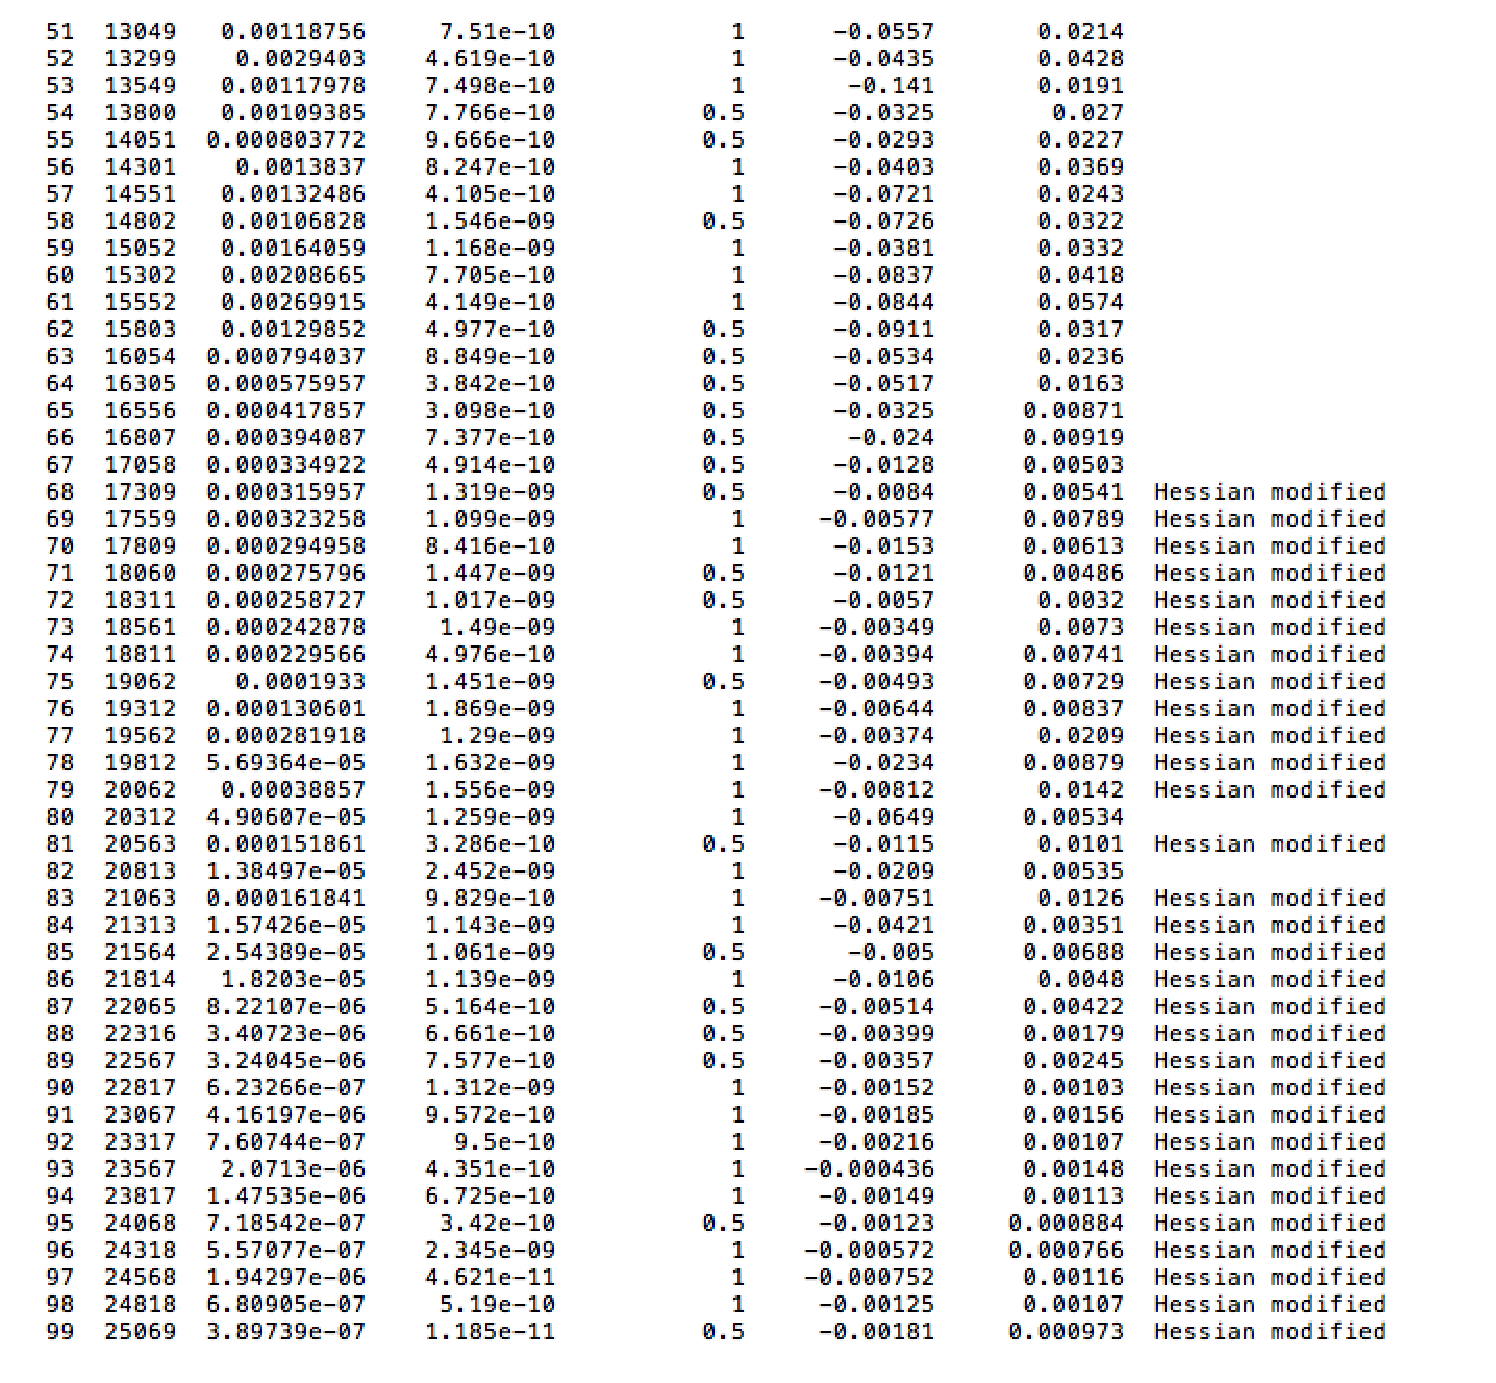
\includegraphics[width=.8\textwidth]{rundata2}
\label{fig:rundata2}
\end{figure}
\chapter{Protein Data Bank Format}
\label{ch:pdb}
\begin{table}[]
\centering
\caption{Explanation of the format of pdb file \cite{pdbformat2}}
\label{tab:pdbformat}
\begin{tabular}{|c|c|c|c|c|}
\hline
\multicolumn{5}{|c|}{Protein Data Bank Format:}                                        \\
\multicolumn{5}{|c|}{Coordinate Section}                                               \\ \hline 
Record Type & Columns & Data                            & Justification & Data Type  \\
ATOM        & 1-4     & ATOM                            &               & character  \\
            & 7-11    & Atom serial number              & right         & integer    \\
            & 13-16   & Atom name                       & left*         & character  \\
            & 17      & Alternate location indicator    &               & character  \\
            & 18-20   & Residue name                    & right         & character  \\
            & 22      & Chain identifier                &               & character  \\
            & 23-26   & Residue sequence number         & right         & integer    \\
            & 27      & Code for insertions of residues &               & character  \\
            & 31-38   & X orthogonal  coordinate       & right         & real (8.3) \\
            & 39-46   & Y orthogonal  coordinate       & right         & real (8.3) \\
            & 47-54   & Z orthogonal  coordinate       & right         & real (8.3) \\
            & 55-60   & Occupancy                       & right         & real (6.2) \\
            & 61-66   & Temperature factor              & right         & real (6.2) \\
            & 73-76   & Segment identifierŚ             & left          & character  \\
            & 77-78   & Element symbol                  & right         & character  \\
            & 79-80   & Charge                          &               & character  \\ \hline
HETATM      & 1-6     & HETATM                          &               & character  \\ 
            & 7-80    & same as ATOM records            &               &            \\ \hline
TER         & 1-3     & TER                             &               & character  \\
            & 7-11    & Serial number                   & right         & integer    \\
            & 18-20   & Residue name                    & right         & character  \\
            & 22      & Chain identifier                &               & character  \\
            & 23-26   & Residue sequence number         & right         & integer    \\
            & 27      & Code for insertions of residues &               & character  \\ \hline
\end{tabular}
\end{table}
\chapter{Cubic Spline}
\label{ch:cubicspline}
The purpose of this chapter is to derive the parameters in the third order polynomial of the cubic spline function. To simplify the derivation, the $x$ point is represented by parameter $t$ where $t$ is from $0$ to $1$. The polynomial is represented by,
\begin{equation}
f_{i}(t)=a_i + b_i t +c_i t^2 +d_i t^3 \qquad i=0,...,n-1
\end{equation} 
Based on the boundary condition where the function should be continuous, 
\begin{align}
\begin{split}
f_{i}(0)&=y_i=a_i \\
f_{i}(1)&=y_{i+1}=a_i+b_i+c_i+d_i.
\end{split}
\end{align}
Another boundary condition is the first derivative should be continous,
\begin{align}
\begin{split}
f_{i}(0)&=D_i=b_i \\
f_{i}(1)&=D_{i+1}=b_i+2 c_i+3 d_i.
\end{split}
\end{align}
Solving for $a_i,b_i,c_i,d_i$ then gives
\begin{align}
\begin{split}
a_i&=y_i \\
b_i &= D_i \\
c_i &= 3 (y_{i+1}-y_i) -2 D_i -D_{i+1} \\
d_i &= 2 (y_i-y_{i+1}) +D_i +D_{i+1}. 
\end{split}
\end{align}
The second derivative should also be continuous,
\begin{align}
\begin{split}
f_{i-1}(1)&=y_i \\
f'_{i-1}(1)&=f'_{i}(0) \\
f_{i}(0)&= y_i \\
f''_{i-1}(1)&=f''_{i}(0). 
\end{split}
\end{align}
To have unique solution, another boundary condition is needed. They are second derivative has to be continous,
\begin{align}
\begin{split}
f_{0}(0)&=y_0 \\
f_{n-1}(1)&=y_n 
\end{split}
\end{align}

A new matrix can be formed based on those constraint. The parameters can be solved using matrix inversion. 
\begin{align}
  \begin{pmatrix}
    2&1& & & &\\
    1&4&1& & &\\
     &1&4&1& &\\
     \vdots&\ddots&\ddots&\ddots&\vdots& \\
     & &1&4&1&\\
     & & &1&2&\\
  \end{pmatrix}
    =
\begin{pmatrix}
    D_{0}\\
    D_{1}\\
    D_{2} \\
    \vdots \\
    D_{n-1} \\
    D_{n}
\end{pmatrix}
\begin{pmatrix}
    3(y_1-y_0)\\
    3(y_2-y_0)\\
    3(y_3-y_1)\\
    \vdots \\
    3(y_n-y_{n-2})\\
    3(y_n-y_{n-1})
   \end{pmatrix}
\end{align}
\end{appendices}
Thus, by inverting the matrix above, the parameters of the interpolation can be determined. In conclusion, the third order polynomial can be used to estimate the value of the function in any point. 
